%!TEX root=../../main.tex
\begin{chapterpage}{Analysis of Variance}
  \chaptertitle{Analysis of Variance}
  \label{ch:ANOVA}
  %/chaptersection{oneSampleMeansWithTDistribution}
  %\chaptersection{pairedData}
  %\chaptersection{differenceOfTwoMeans}
  %\chaptersection{PowerForDifferenceOfTwoMeans}
  \chaptersection{anovaAndRegrWithCategoricalVariables}
  \chaptersection{multipleComparisonsAndControllingTheType1ErrorRate}
  %\chaptersection{inferenceForNumericalDataNotes}
  \chaptersection{ANOVAExercises}
\end{chapterpage}
\renewcommand{\chapterfolder}{ch_inference_for_means_oi_biostat}

\chapterintro{
  In some settings, it is useful to compare means across several groups. It might be tempting to do pairwise comparisons between groups; for example, if there are three groups ($A, B, C$), why not conduct three separate $t$-tests ($A$ vs. $B$, $A$ vs. $C$, $B$ vs. $C$)?

  The primary issue here is that we are inspecting the data before picking the groups that will be compared. It is inappropriate to examine all data by eye (informal testing) and only afterwards decide which parts to formally test. This is called \term{data snooping} or \term{data fishing}. Naturally we would pick the groups with the large differences for the formal test, leading to an inflation in the Type 1 Error rate. To understand this better, let's consider the following problem:

Suppose we are to measure the aptitude for students in 20 classes in a large elementary school at the beginning of the year. In this school, all students are randomly assigned to classrooms, so any differences we observe between the classes at the start of the year are completely due to chance. However, with so many groups, we will probably observe a few groups that look rather different from each other. If we select only these classes that look so different, we will probably make the wrong conclusion that the assignment wasn't random. While we might only formally test differences for a few pairs of classes, we informally evaluated the other classes by eye before choosing the most extreme cases for a comparison.
 For additional information on the ideas expressed in this example, we recommend reading about the \term{prosecutor's fallacy}.\footnote{See, for example, \href{http://www.stat.columbia.edu/~cook/movabletype/archives/2007/05/the_prosecutors.html}{www.stat.columbia.edu/$\sim$cook/movabletype/archives/2007/05/the\_prosecutors.html}.}



In the next section we will learn how to use the $F$ statistic and ANOVA to test whether observed differences in means could have happened just by chance even if there was no difference in the respective population means. 
  Conducting multiple tests on the same data increases the rate of Type I error, making it more likely that a difference will be found by chance, even if there is no difference among the population means. Multiple testing is discussed further in Section~\ref{multipleComparisonsAndControllingTheType1ErrorRate}.

}


%_____________
\section{Comparing means with ANOVA}
\label{anovaAndRegrWithCategoricalVariables}

\index{analysis of variance (ANOVA)|(}



Instead, the methodology behind a $t$-test can be generalized to a procedure called \term{analysis of variance (ANOVA)}, which uses a single hypothesis test to assess whether the means across several groups are equal. Strong evidence favoring the alternative hypothesis in ANOVA is described by unusually large differences among the group means.

\begin{itemize}
	\setlength{\itemsep}{0mm}
	\item[$H_0$:] The mean outcome is the same across all $k$ groups. In statistical notation, $\mu_1 = \mu_2 = \cdots = \mu_k$ where $\mu_i$ represents the mean of the outcome for observations in category $i$.
	\item[$H_A$:] At least one mean is different.
\end{itemize}

There are three conditions on the data that must be checked before performing ANOVA: 1) observations are independent within and across groups, 2) the data within each group are nearly normal, and 3) the variability across the groups is about equal.

\begin{examplewrap}
\begin{nexample}{Examine Figure~\ref{toyANOVA}. Compare groups I, II, and III. Is it possible to visually determine if the differences in the group centers is due to chance or not? Now compare groups IV, V, and VI. Do the differences in these group centers appear to be due to chance?}		
It is difficult to discern a difference in the centers of groups I, II, and III, because the data within each group are quite variable relative to any differences in the average outcome. However, there appear to be differences in the centers of groups IV, V, and VI. For instance, group V appears to have a higher mean than that of the other two groups. The differences in centers for groups IV, V, and VI are noticeable because those differences are large relative to the variability in the individual observations within each group.
\end{nexample}
\end{examplewrap}

\begin{figure}[h]
	\centering
	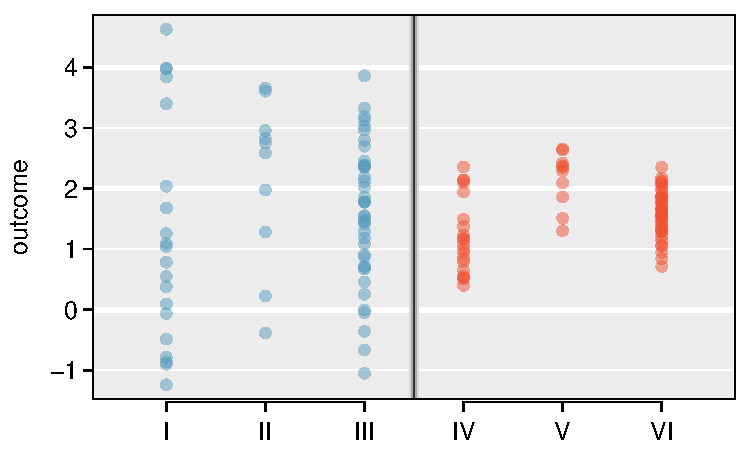
\includegraphics[width=0.68\textwidth]{ch_07a_inference_for_means_oi_biostat/figures/toyANOVA/toyANOVA}
	\caption{Side-by-side dot plot for the outcomes for six groups.}
	\label{toyANOVA}
\end{figure}		

\subsection{Diagnostics for ANOVA}

%\textD{\newpage}
As we have said, there are three conditions we must check for an ANOVA analysis: all observations must be independent, the data in each group must be nearly normal, and the variance within each group must be approximately equal.

\begin{description}
\item[Independence.] If the data are a simple random sample from less
  than 10\% of the population, this condition is satisfied.  If the
  group is assigned, of instance, in a clinical trial, then the group
  should be randomly  asssigned. 
\item[Approximately normal.] As with one- and two-sample testing for
  means, the normality assumption is especially important when the
  sample size is quite small. Techniques to check that a
  distribution is normal are \term{Shapiro--Wilk} test,
  \term{Kolmogorov--Smirnov} 
  test or Q-Q plot. Sometimes in ANOVA there are so many groups or so few observations per group that checking normality for each group isn't reasonable. For groups with a sample size large enough, namely greater than 30, the normal condition is not needed to be tested by these techniques.

\item[Constant variance.] The last assumption is that the variance in
  the groups is about equal from one group to the next. A method to check the
  constant variance is applying the \term{Levene's test}. 


\end{description}


\subsection{Analysis of variance (ANOVA) and the $\pmb{F}$-test}
\label{ANOVASection}

\noindent%
The \data{famuss} dataset was introduced in Chapter~\ref{introductionToData}, Section~\ref{variableTypes}. In the FAMuSS study, researchers examined the relationship between muscle strength and genotype at a location on the ACTN3 gene. The measure for muscle strength is percent change in strength in the non-dominant arm (\var{ndrm.ch}). Is there a difference in muscle strength across the three genotype categories (\texttt{CC}, \texttt{CT},~\texttt{TT})?

\begin{exercisewrap}
\begin{nexercise}\label{nullHypForFamuss}%
The null hypothesis under consideration is the following: $\mu_{\resp{CC}} = \mu_{\resp{CT}} = \mu_{\resp{TT}}$.
Write the null and corresponding alternative hypotheses in plain language.\footnotemark{}
\end{nexercise}
\end{exercisewrap}
\footnotetext{$H_0$: The average percent change in non-dominant arm strength is equal across the three genotypes. $H_A$: The average percent change in non-dominant arm strength varies across some (or all) groups.}

Figure~\ref{famussSummaryTable} provides summary statistics for each group. A side-by-side boxplot for the change in non-dominant arm strength is shown in Figure~\ref{famussBoxPlot_2nd}; Figure~\ref{famussNormal} shows the Q-Q plots by each genotype. Notice that the variability appears to be approximately constant across groups; nearly constant variance across groups is an important assumption that must be satisfied for using ANOVA. Based on the Q-Q plots, there is evidence of moderate right skew; the data do not follow a normal distribution very closely, but could be considered to 'loosely' follow a normal distribution.\footnote{In a more advanced course, it can be shown that the ANOVA procedure still holds with deviations from normality when sample sizes are moderately large. Additionally, a more advanced course would discuss appropriate transformations to induce normality.} It is reasonable to assume that the observations are independent within and across groups; it is unlikely that participants in the study were related, or that data collection was carried out in a way that one participant's change in arm strength could influence another's. 

\begin{figure}[ht]
	\centering\small
	\begin{tabular}{lrrr}
		\hline
		& \resp{CC} & \resp{CT} & \resp{TT} \\
		\hline
		Sample size ($n_i$)	& 173 & 261 & 161 \\
		Sample mean ($\bar{x}_i$)	& 48.89 & 53.25 & 58.08 \\
		Sample SD ($s_i$)	& 29.96 & 33.23 & 35.69 \\
		\hline
	\end{tabular}
	\caption{Summary statistics of change in non-dominant arm strength, split by genotype.}
	\label{famussSummaryTable}
\end{figure}


\begin{figure}[h]
	\centering
	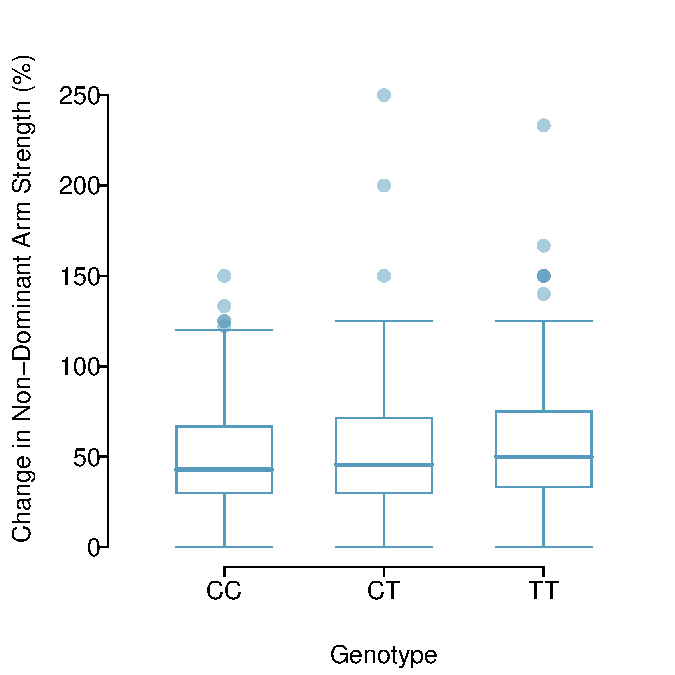
\includegraphics[width=0.475\textwidth]{ch_07a_inference_for_means_oi_biostat/figures/famussBoxPlot/famussBoxPlot}
	\caption{Side-by-side box plot of the change in non-dominant arm strength for 595 participants across three groups.}
	\label{famussBoxPlot_2nd}
\end{figure}

\begin{figure}[h]
	\centering
	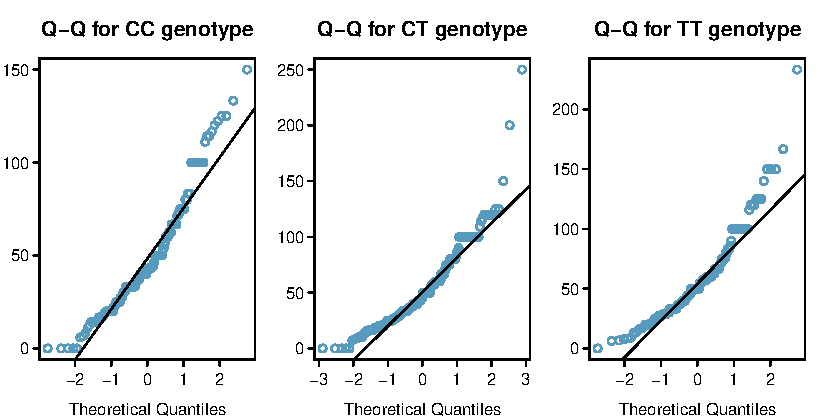
\includegraphics[width=\textwidth]{ch_07a_inference_for_means_oi_biostat/figures/famussNormal/famussNormal}
	\caption{Q-Q plots of the change in non-dominant arm strength for 595 participants across three groups.}
	\label{famussNormal}
\end{figure}


\begin{examplewrap}
\begin{nexample}{The largest difference between the sample means is between the \texttt{CC} and \texttt{TT} groups. Consider again the original hypotheses:
		\begin{itemize}
			\setlength{\itemsep}{0mm}
			\item[$H_0$:] $\mu_{\resp{CC}} = \mu_{\resp{CT}} = \mu_{\resp{TT}}$
			\item[$H_A$:] The average percent change in non-dominant arm strength ($\mu_i$) varies across some (or all) groups.
		\end{itemize}
		Why might it be inappropriate to run the test by simply estimating whether the difference of $\mu_{\var{CC}}$ and $\mu_{\resp{TT}}$ is statistically significant at a 0.05 significance level?}\label{multipleComparisonExample}%	
It is inappropriate to informally examine the data and decide which groups to formally test. This is a form of \term{data fishing}; choosing the groups with the largest differences for the formal test will lead to an increased chance of incorrectly rejecting the null hypothesis (i.e., an inflation in the Type~I error rate). Instead, all the groups should be tested using a single hypothesis test.
\end{nexample}
\end{examplewrap}

Analysis of variance focuses on answering one question: is the variability in the sample means large enough that it seems unlikely to be from chance alone? The variation between groups is referred to as the \term{mean square between groups ($MSG$)}; the $MSG$ is a measure of how much each group mean varies from the overall mean. Let $\overline{x}$ represent the mean of outcomes across all groups, where $\overline{x}_i$ is the mean of outcomes in a particular group $i$ and $n_i$ is the sample size of group $i$. The mean square between groups is:
\[MSG = \frac{1}{k-1}\sum_{i=1}^{k} n_{i}\left(\overline{x}_{i} - \overline{x}\right)^{2} = \frac{1}{\textrm{df}_{G}}SSG,\] 
where $SSG$ is the \term{sum of squares between groups}, $\sum_{i=1}^{k} n_{i}\left(\overline{x}_{i} - \overline{x}\right)^{2}$, and $\textrm{df}_{G}=k-1$ is the degrees of freedom associated with the $MSG$ when there are $k$ groups.

%\textD{\newpage}

Under the null hypothesis, any observed variation in group means is due to chance and there is no real difference between the groups. In other words, the null hypothesis assumes that the groupings are non-informative, such that all observations can be thought of as belonging to a single group. If this scenario is true, then it is reasonable to expect that the variability between the group means should be equal to the variability observed within a single group. The \term{mean square error ($MSE$)} is a pooled variance estimate with associated degrees of freedom $\textrm{df}_E=n-k$ that provides a measure of variability within the groups. The mean square error is computed as:
\[MSE = \frac{1}{n-k}\sum_{i=1}^{k} (n_i-1)s_i^{2} = \frac{1}{\textrm{df}_{E}}SSE, \]
where the $SSE$ is the \term{sum of squared errors}, $n_i$ is the sample size of group $i$, and $s_i$ is the standard deviation of group $i$.

Under the null hypothesis that all the group means are equal, any differences among the sample means are only due to chance; thus, the $MSG$ and $MSE$ should also be equal. ANOVA is based on comparing the $MSG$ and $MSE$. The test statistic for ANOVA, the \term{F-statistic}, is the ratio of the between-group variability to the within-group variability:
\begin{align}
\label{formulaForTheFStatistic}%
F = \frac{MSG}{MSE}.
\end{align}

\begin{examplewrap}
\begin{nexample}{Calculate the $F$-statistic for the \data{famuss} data summarized in Figure~\ref{famussSummaryTable}. The overall mean $\overline{x}$ across all observations is 53.29.}
 
First, calculate the $MSG$ and $MSE$. 
\vspace{0mm}
\begin{align*}
MSG =& \frac{1}{k-1}\sum_{i=1}^{k} n_{i}\left(\bar{x}_{i} - \bar{x}\right)^{2} \\
=& \frac{1}{3-1} [(173)(48.89 - 53.29)^{2} + (261)(53.25 - 53.29)^{2} + (161)(58.08 - 53.29)^{2} ]\\
=& 3521.69 \\
MSE =& \frac{1}{n-k}\sum_{i=1}^{k} (n_i-1)s_i^{2} \\
=& \frac{1}{595-3}[(173-1)(29.96^2) + (261-1)(33.23^2) + (161-1)(35.69^2)] \\
=& 1090.02
\end{align*}

The $F$-statistic is the ratio:

\[\dfrac{MSG}{MSE} = \dfrac{3521.69}{1090.02} = 3.23. \]
\end{nexample}
\end{examplewrap} 

%\textD{\newpage}

A $p$-value can be computed from the $F$-statistic using an $F$-distribution, which has two associated parameters: $\textrm{df}_{1}$ and $\textrm{df}_{2}$. For the $F$-statistic in ANOVA, $\textrm{df}_{1} = \textrm{df}_{G}$ and $\textrm{df}_{2}= \textrm{df}_{E}$. An $F$ distribution with 2 and 592 degrees of freedom, corresponding to the $F$-statistic for the genotype and muscle strength hypothesis test, is shown in Figure~\ref{fDist2And592Shaded}.

\begin{figure}[ht]
	\centering
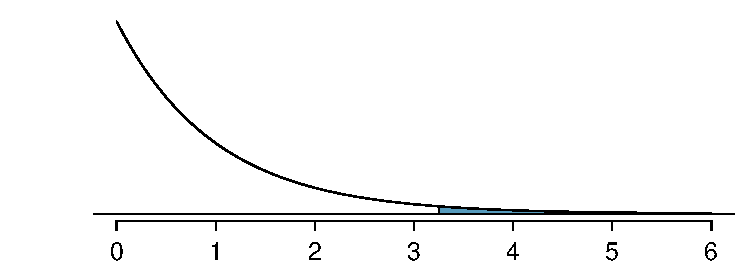
\includegraphics[width=0.65\textwidth]{ch_07a_inference_for_means_oi_biostat/figures/fDist2And592/fDist2And592Shaded}
	\caption{An $F$-distribution with $\textrm{df}_1=2$ and $\textrm{df}_2=592$. The tail area greater than $F = 3.23$ is shaded.}
	\label{fDist2And592Shaded}
\end{figure}

The larger the observed variability in the sample means ($MSG$) relative to the within-group variability ($MSE$), the larger $F$ will be. Larger values of $F$ represent stronger evidence against the null hypothesis. The upper tail of the distribution is used to compute a $p$-value, which is typically done using statistical software.

\begin{examplewrap}
\begin{nexample}{The $p$-value corresponding to the test statistic is equal to about 0.04. Does this provide strong evidence against the null hypothesis at significance level $\alpha = 0.05$?}
The $p$-value is smaller than 0.05, indicating the evidence is strong enough to reject the null hypothesis at a significance level of 0.05. The data suggest that average change in strength in the non-dominant arm varies by participant genotype.	
\end{nexample}
\end{examplewrap}

\begin{onebox}{The $\pmb{F}$-statistic and the $\pmb{F}$-test}
		Analysis of variance (ANOVA) is used to test whether the mean outcome differs across two or more groups. ANOVA uses a test statistic $F$, which represents a standardized ratio of variability in the sample means relative to the variability within the groups. If $H_0$ is true and the model assumptions are satisfied, the statistic $F$ follows an $F$ distribution with parameters $\textrm{df}_{1}=k-1$ and $\textrm{df}_{2}=n-k$. The upper tail of the $F$-distribution is used to calculate the $p$-value.
\end{onebox}


%\textD{\newpage}


\subsection{Reading an ANOVA table from software}

The calculations required to perform an ANOVA by hand are tedious and prone to human error. Instead, it is common to use statistical software to calculate the $F$-statistic and associated $p$-value.
%The results of an ANOVA can be summarized in a table similar to that of a regression summary, which will be discussed in Chapters~\ref{linRegrForTwoVar} and~\ref{multipleLinearRegression}.

Figure~\ref{anovaSummaryTableForFamuss} shows an ANOVA summary to test whether the mean change in non-dominant arm strength varies by genotype. Many of these values should look familiar; in particular, the $F$-statistic and $p$-value can be retrieved from the last two columns.
\textD{\vspace{5mm}}

\begin{figure}[ht]
	\centering
	\begin{tabular}{lrrrrr}
		\hline
		& Df & Sum Sq & Mean Sq & F value & Pr($>$F) \\ 
		\hline
		famuss\$actn3.r577x & 2 & 7043 & 3522 & 3.231 & 0.0402 \\ 
		Residuals & 592 & 645293 & 1090 &  &  \\    \hline
	\end{tabular}
	\caption{ANOVA summary for testing whether the mean change in non-dominant arm strength varies by genotype at the \texttt{actn3.r577x} location on the ACTN3 gene.}
	\label{anovaSummaryTableForFamuss}
\end{figure}

\subsection{An example with R-Commander}

\begin{figure}
  \centering
  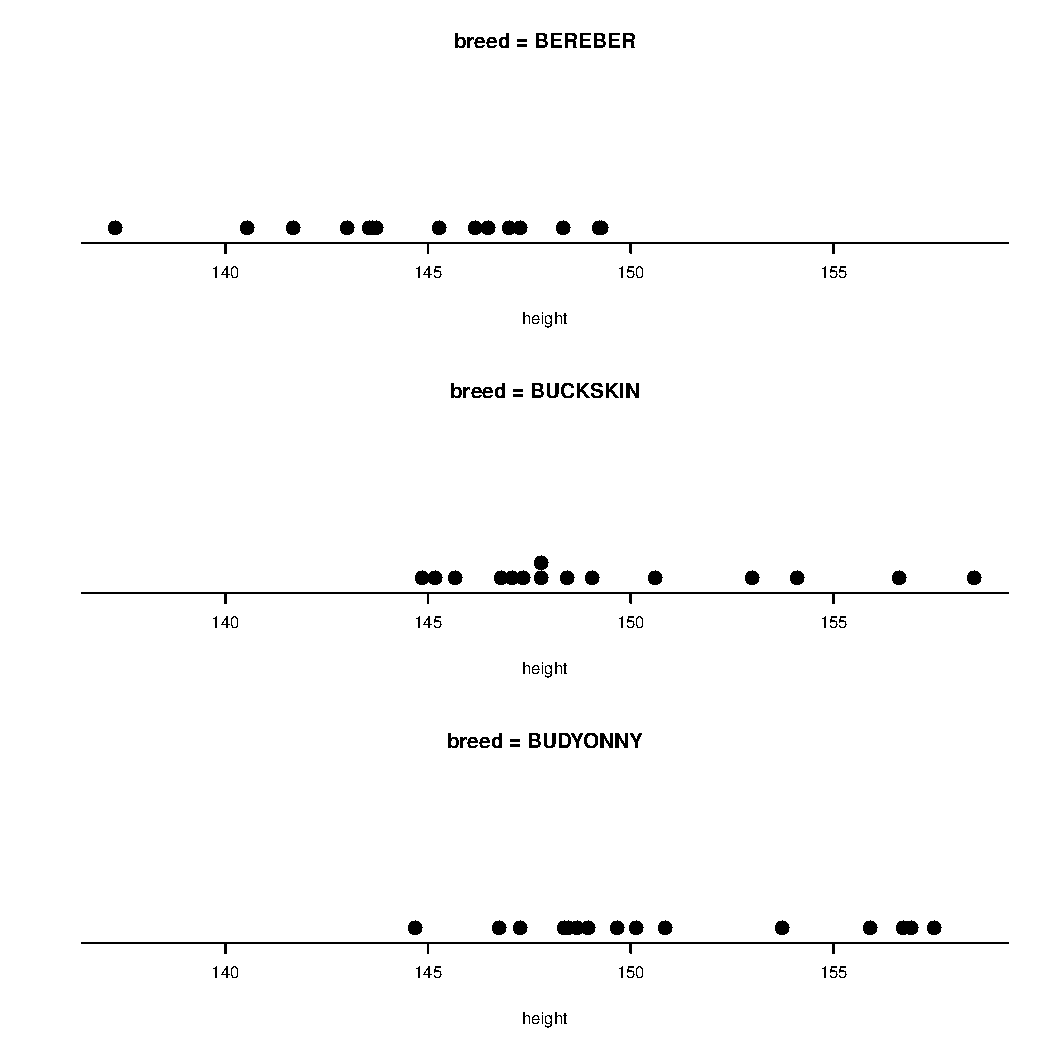
\includegraphics[width=0.8\textwidth]{ch_07a_inference_for_means_oi_biostat/figures/horses/ComparingValues.pdf}
\caption{Distribution of height within each breed.}
\label{fig:horse_breed}
\end{figure}

\begin{example}{
An ethnology research group wants to determine whether or not there exist
       significant differences from  the height of horses depending on the
       breed. For this purpose, 45 horses have been  chosen
       belonging to three different breeds (Berber, Buckskin and
       Budyonny) and they have been randomly selected  in such a way
       there are 15 horses for each breed. In
       Figure~\ref{fig:horse_breed} the height of the horses is
       displayed for each group. 

     }

     \begin{description}
     \item[Condition 1: Independence] 
     
   This hypothesis is fulfilled, since the assignment of the treatment
 has been randomized across the breeds. 
 The text explains that the horses have been randomly selected among the
 horses of the same breed.
  \item[Condition 2: Normality ] 
  The hypotheses of the normality of Berber horses  are:
    \begin{tabular}{ll}
      $H_0$ : & The height is normally distributed for breed Berber \\
$H_A $: &  The height is not normally distributed for breed Berber 
    \end{tabular}
     
According to the data shown in the figure~\ref{fig:ShapiroHorses}, the p-value 0.5754 is greater than $\alpha=0.05$. Hence, we fail to
reject the null hypothesis and a normal distribution of height  for
Berber horses.
The corresponding p-values for Buckskin and Budyonny breeds are
0.05096 and  0.1076, respectively. 
\item[Levene's test (identical variances) ]
    The hypotheses of the variances of the height of the horses are: \newline
  \begin{tabular}{ll}
    $H_0$ & $\sigma_{Berber}^2=\sigma_{Buckskin}^2=\sigma_{Budyonny}^2$ \\
    $H_A$ & $\sigma_{Berber}^2\neq \sigma_{Buckskin}^2$ or
            $\sigma_{Berber}^2 \neq \sigma_{Budyonny}^2$ or
            $\sigma_{Buckskin}^2\neq \sigma_{Budyonny}^2$ 
  \end{tabular} \newline
  where $\sigma_{Berber}^2$ is the population variance of the height
  of Berber horses.
  
  According to the figure~\ref{fig:LeveneHorses},  T
 the p-value=0.8564 is greater than $\alpha=0.05$
We fail to reject the null hypothesis and we do not have evidence against being any difference among the variances. 
We can assume that for the three breeds  have identical variance. 
\end{description}
Finally, we can perform the ANOVA test, since all the conditions are
met.

The hypotheses of the ANOVA test are: \newline
  \begin{tabular}{ll}
    $H_0$ & $\mu_{Berber}=\mu_{Buckskin}=\mu_{Budyonny}$ \\
    $H_A$ & $\mu_{Berber}\neq \mu_{Buckskin}$ or
            $\mu_{Berber} \neq \mu_{Budyonny}$ or
            $\mu_{Buckskin}\neq \mu_{Budyonny}$ 
  \end{tabular}\newline
  where $\mu_{Berber}$ is the population mean of the height
  of Berber horses and analogously for the other groups.
  
       The degrees of freedom are  $k-1=3-1=2$ and $n-k=45-3=42$.
The significance level is $\alpha=0.05$. Hence, we use 95 percentile
for the Snedecor's F-table with degrees of freedom 2 and 50,which is
the closest
value to 42 in the table, the value is $F_{2,50,0.95}=3.18$. The acceptance interval is $[0, 3.18)$. 

  
  


The test statistic $F=10.1$ is outside interval we reject null
hypothesis. We have enough evidence that the height of horses depends
on the breed. Please, observe that the computer (figure~\ref{fig:ANOVAhorses})  provides a more accurate 
p-value and the test statistic. 
\end{example}
\begin{figure}
  \centering
  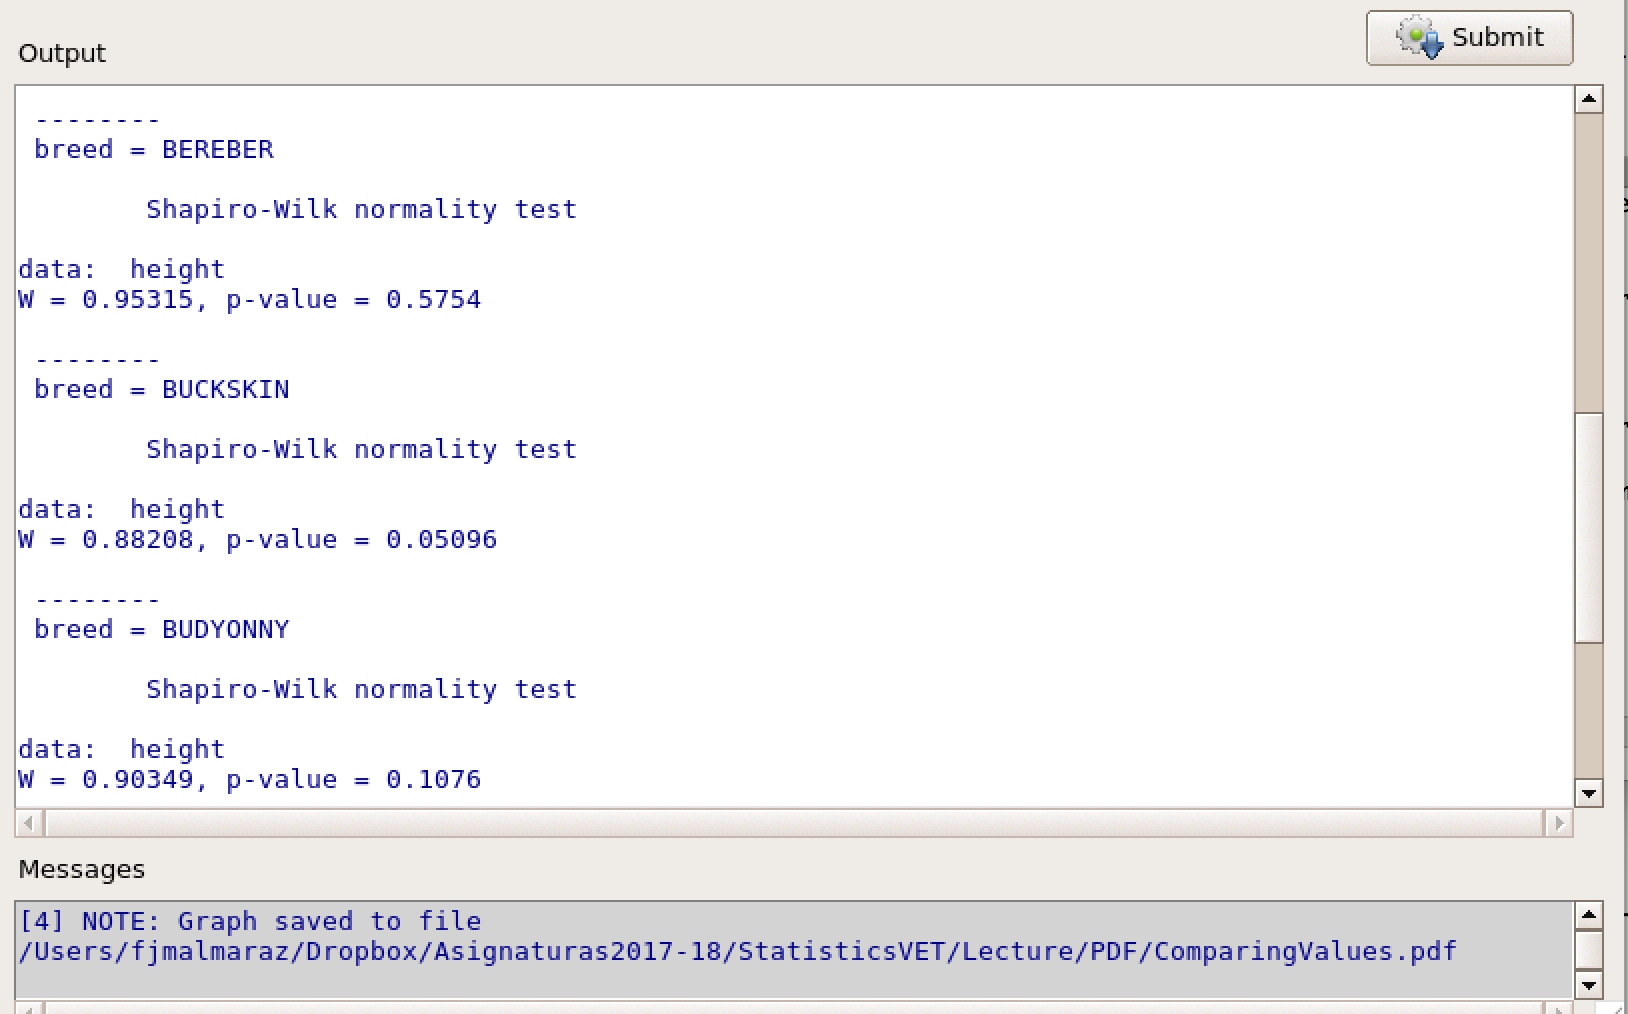
\includegraphics[width=0.95\textwidth]{ch_07a_inference_for_means_oi_biostat/figures/horses/ShapiroHorses.png}
\caption{Screenshot of Shapiro-Wilk test.}
\label{fig:ShapiroHorses}
\end{figure}
\begin{figure}
  \centering
   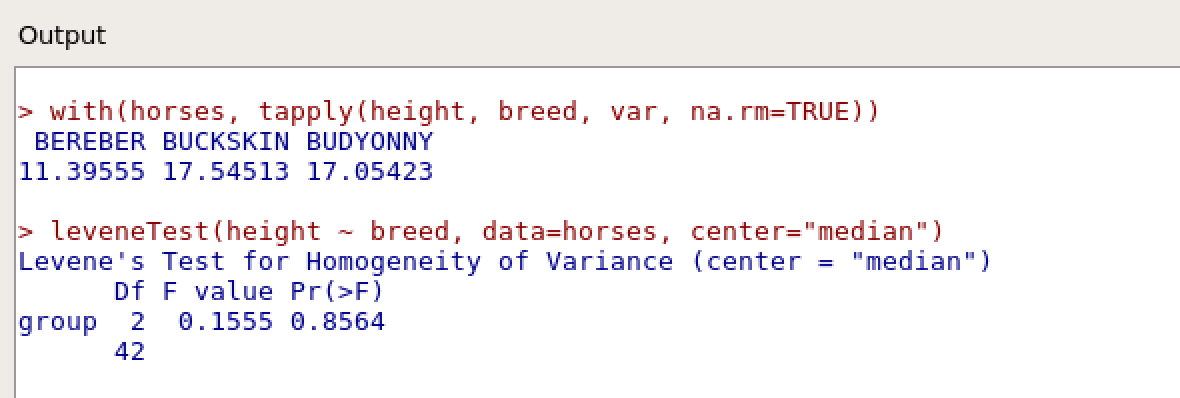
\includegraphics[width=0.95\textwidth]{ch_07a_inference_for_means_oi_biostat/figures/horses/LeveneHorses.png}
\caption{Screenshot of Levene's test. .}
\label{fig:LeveneHorses}
\end{figure}

\begin{figure}
  \centering
  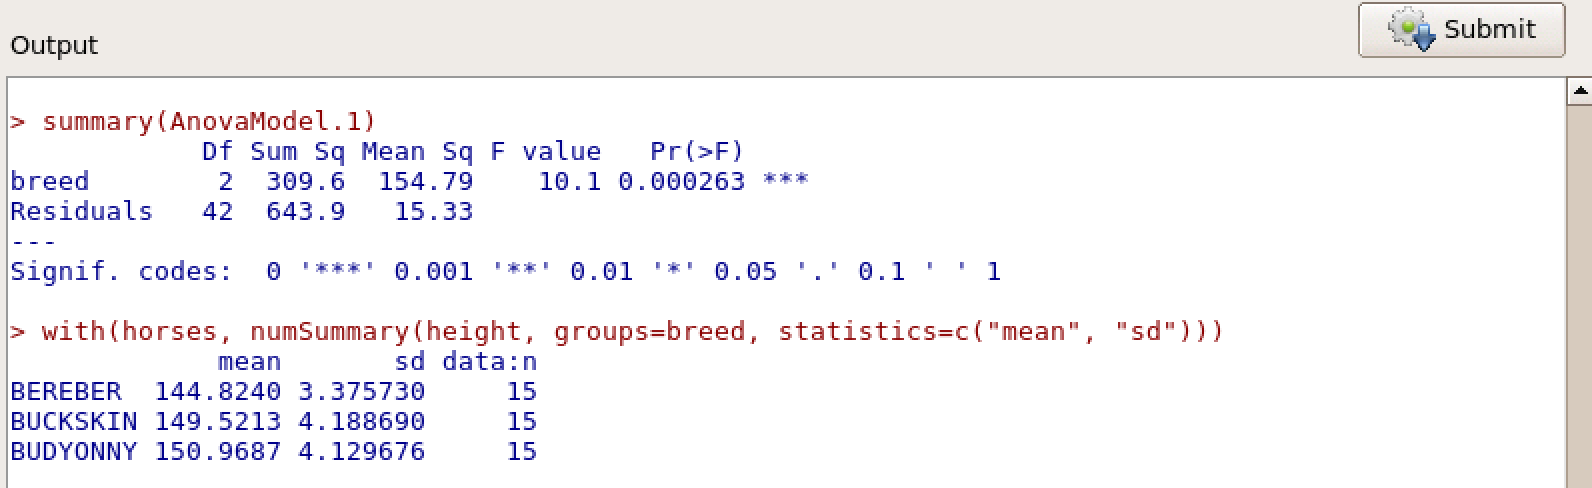
\includegraphics[width=0.95\textwidth]{ch_07a_inference_for_means_oi_biostat/figures/horses/ANOVAhorses.png}
\caption{Screenshot of ANOVA test .}
\label{fig:ANOVAhorses}
\end{figure}




\section{Multiple comparisons and controlling Type~I Error rate}
\label{multipleComparisonsAndControllingTheType1ErrorRate}

\index{significance level!multiple comparisons|(}

Rejecting the null hypothesis in an ANOVA analysis only allows for a conclusion that there is evidence for a difference in group means. In order to identify the groups with different means, it is necessary to perform further testing. For example, in the \data{famuss} analysis, there are three comparisons to make: \resp{CC} to \resp{CT}, \resp{CC} to \resp{TT}, and \resp{CT} to \resp{TT}. While these comparisons can be made using two sample $t$-tests, it is important to control the Type I error rate. One of the simplest ways to reduce the overall probability of identifying a significant difference by chance in a multiple comparisons setting is to use the Bonferroni correction procedure.

In the Bonferroni correction procedure, the $p$-value from a two-sample $t$-test is compared to a modified significance level, $\alpha^\star$; $\alpha^\star = \alpha/K$, where $K$ is the total number of comparisons being considered. For $k$ groups, $K=\frac{k(k-1)}{2}$. When calculating the $t$-statistic, use the pooled estimate of standard deviation between groups (which equals $\sqrt{MSE}$); to calculate the $p$-value, use a $t$-distribution with $\textrm{df}_2$. It is typically more convenient to do these calculations using software. 

\begin{onebox}{Bonferroni correction}
The \term{Bonferroni correction} suggests that a more stringent significance level is appropriate when conducting multiple tests:
\begin{align*}
\alpha^\star = \alpha / K
\end{align*}
where $K$ is the number of comparisons being considered. For $k$ groups, $K=\frac{k(k-1)}{2}$.
\end{onebox}

\begin{examplewrap}
\begin{nexample}{The ANOVA conducted on the \data{famuss} dataset showed strong evidence of differences in the mean strength change in the non-dominant arm between the three genotypes. Complete the three possible pairwise comparisons using the Bonferroni correction and report any differences.}

Use a modified significance level of $\alpha^\star = 0.05/3 = 0.0167$. The pooled estimate of the standard deviation is $\sqrt{MSE} = \sqrt{1090.02} = 33.02$.

Genotype \resp{CC} versus Genotype \resp{CT}: 
\[
t = \frac{\overline{x}_1 - \overline{x}_2}{s_{\text{pooled}}\sqrt{\frac{1}{n_1} + \frac{1}{n_2}}} 
 = \dfrac{48.89 - 53.25}{33.02 \sqrt{\frac{1}{173} + \frac{1}{261}}} = -1.35.\]
 
This results in a $p$-value of 0.18 on $df =592$. This $p$-value is larger than $\alpha^\star = 0.0167$, so there is not evidence of a difference in the means of genotypes \resp{CC} and \resp{CT}.

Genotype \resp{CC} versus Genotype \resp{TT}: 
 \[
 t = \frac{\overline{x}_1 - \overline{x}_2}{s_{\text{pooled}}\sqrt{\frac{1}{n_1} + \frac{1}{n_2}}}
 = \dfrac{48.89 - 58.08}{33.02 \sqrt{\frac{1}{173} + \frac{1}{161}}} = -2.54.\]

This results in a $p$-value of 0.01 on $df =592$. This $p$-value is smaller than $\alpha^\star = 0.0167$, so there is evidence of a difference in the means of genotypes \resp{CC} and \resp{TT}.
 
Genotype \resp{CT} versus Genotype \resp{TT}:  
 \[
 t = \frac{\overline{x}_1 - \overline{x}_2}{s_{\text{pooled}}\sqrt{\frac{1}{n_1} + \frac{1}{n_2}}}
 = \dfrac{53.25 - 58.08}{33.02 \sqrt{\frac{1}{261} + \frac{1}{161}}} = -1.46.\]

This results in a $p$-value of 0.14 on $df =592$. This $p$-value is larger than $\alpha^\star = 0.0167$, so there is not evidence of a difference in the means of genotypes \resp{CT} and \resp{TT}.

In summary, the mean percent strength change in the non-dominant arm for genotype \resp{CT} individuals is not statistically distinguishable from those of genotype \resp{CC} and \resp{TT} individuals. However, there is evidence that mean percent strength change in the non-dominant arm differs between individuals of genotype \resp{CC} and \resp{TT} are different. 
\end{nexample}
\end{examplewrap}

\index{significance level!multiple comparisons|)}
\index{analysis of variance (ANOVA)|)}


%\textD{\newpage}


\subsection{Reading the results of pairwise $\pmb{\MakeLowercase{t}}$-tests from software}

Statistical software can be used to calculate the $p$-values associated with each possible pairwise comparison of the groups in ANOVA. The results of the pairwise tests are summarized in a table that shows the $p$-value for each two-group test. 

Figure~\ref{posthocTestsForFamussUnadjusted} shows the $p$-values from the three possible two-group $t$-tests comparing change in non-dominant arm strengths between individuals with genotypes \texttt{CC}, \texttt{CT}, and \texttt{TT}. For example, the table indicates that when comparing mean change in non-dominant arm strength between \texttt{TT} and \texttt{CC} individuals, the $p$-value is 0.01. This coheres with the calculations above, and these unadjusted $p$-values should be compared to $\alpha^\star = 0.0167$.

% latex table generated in R 3.6.2 by xtable 1.8-4 package
% Tue Jun 09 12:34:41 2020
\begin{figure}[ht]
	\centering
	\begin{tabular}{rrr}
		\hline
		& CC & CT \\ 
		\hline
		CT & 0.18 &  - \\ 
		TT & 0.01 & 0.14 \\ 
		\hline
	\end{tabular}
	\caption{Unadjusted $p$-values for pairwise comparisons testing whether the mean change in non-dominant arm strength varies by genotype at the \texttt{actn3.r577x} location on ACTN3 gene.} 
	\label{posthocTestsForFamussUnadjusted}
\end{figure}

The use of statistical software makes it easier to apply corrections for multiple testing, such that it is not necessary to explicitly calculate the value of $\alpha^\star$. Figure~\ref{posthocTestsForFamussAdjusted} shows the Bonferroni-adjusted $p$-values from the three possible tests. When statistical software applies the Bonferroni correction, the unadjusted $p$-value is multiplied by $K$, the number of comparisons, allowing for the values to be directly compared to $\alpha$, not $\alpha^\star$. Comparing an unadjusted $p$-value to $\alpha/K$ is equivalent to comparing the quantity $(K \times p\text{-value})$ to $\alpha$.

\begin{figure}[ht]
	\centering
	\begin{tabular}{rrr}
		\hline
		& CC & CT \\ 
		\hline
		CT & 0.54 &  - \\ 
		TT & 0.03 & 0.43 \\ 
		\hline
	\end{tabular}
	\caption{Bonferroni-adjusted $p$-values for pairwise comparisons testing whether the mean change in non-dominant arm strength varies by genotype at the \texttt{actn3.r577x} location on ACTN3 gene.} 
	\label{posthocTestsForFamussAdjusted}
\end{figure}


\subsection{Tuckey's range test}


Another technique to compare which pairs of groups are significantly different is
the Tuckey's range test, where a confidence interval is given for a
pairwise comparison. If zero is not included in the confidence
interval, we have enough evidence of a significant difference between the two
groups. An example with the breeds of horses is in the figure~\ref{fig:Tuckey}

\begin{figure}
\centering
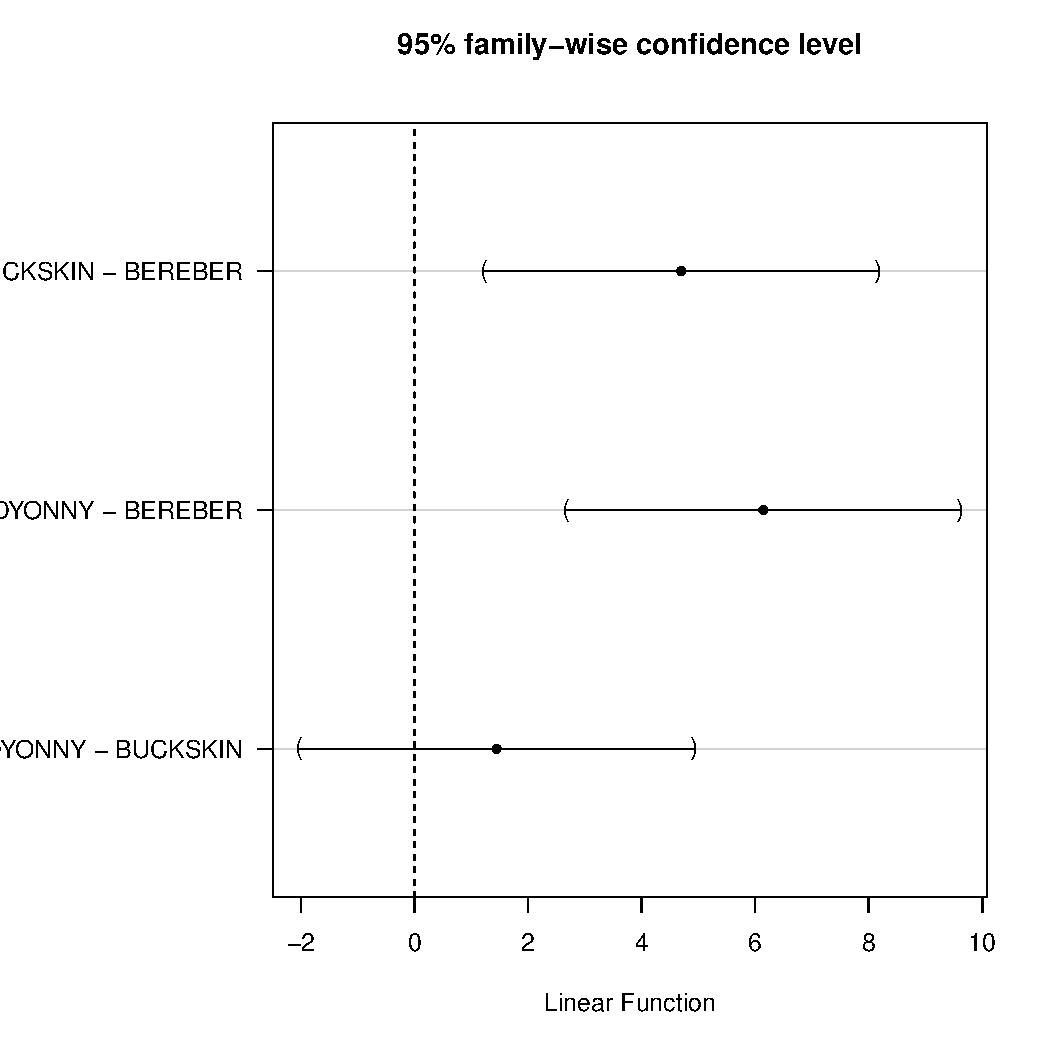
\includegraphics[width=0.8\textwidth]{ch_07a_inference_for_means_oi_biostat/figures/horses/Tuckey}
\caption{.Tuckey's confidence interval for pairwise comparison.  We have evidence of a difference between Berber and the other
      two breeds, since the zero value is not included in the interval. However, we do not have enough evidence that there
      exists a difference of mean  between Budyonny and Buckskin. }
\label{fig:Tuckey}
\end{figure}
\begin{caution}
{Sometimes an ANOVA will reject the null but no groups will have statistically significant differences}
{It is possible to reject the null hypothesis using ANOVA and then to not subsequently identify differences in the pairwise comparisons. However, \emph{this does not invalidate the ANOVA conclusion}. It only means we have not been able to successfully identify which groups differ in their means.}
\end{caution}

The ANOVA procedure examines the big picture: it considers all groups simultaneously to decipher whether there is evidence that some difference exists. Even if the test indicates that there is strong evidence of differences in group means, identifying with high confidence a specific difference as statistically significant is more difficult.

Consider the following analogy: we observe a Wall Street firm that makes large quantities of money based on predicting mergers. Mergers are generally difficult to predict, and if the prediction success rate is extremely high, that may be considered sufficiently strong evidence to warrant investigation by the Securities and Exchange Commission (SEC). While the SEC may be quite certain that there is insider trading taking place at the firm, the evidence against any single trader may not be very strong. It is only when the SEC considers all the data that they identify the pattern. This is effectively the strategy of ANOVA: stand back and consider all the groups simultaneously.
